\documentclass{article}
\usepackage{graphicx}
\usepackage{fullpage}
\usepackage{float}
\title{Implementation of the exponential function}
\author{H.H.Nielsen}
\date{}
\begin{document}
\maketitle

\begin{abstract}
A "quick-and-dirty" implementation of the exponential function introduced
and explained. A test is also included.
\end{abstract}

\section{Code implementation}
The code is implemented in the following way:

	{double ex(double x)
		
	if(x$<$0)return 1/ex(-x);

	if(x$>$1./8)return pow(ex(x/2),2);

	return 1+x*(1+x/2*(1+x/3*(1+x/4*(1+x/5*(1+x/6*(1+x/7*(1+x/8*(1+x/9*(1+x/10)))))))));


The code takes a double value, x, and returns an approximate value of:

	\begin{equation}\label{eq:exp}
		f(x) = e^x \;.
	\end{equation}


\section{Explanation}
The first line inside the function makes sure no values of negative signs
are included in the summation. The second line returns the square of e$^{x/2}$ 
if the x value is larger than 0.125. This ensures that only small values of x
are calculated with the Taylor expansion in the third line.
The Taylor expansion is defined as~\cite{taylor},
	\begin{equation}\label{eq:nemes}
\exp x := \sum_{k = 0}^{\infty} \frac{x^k}{k!} = 1 + x + \frac{x^2}{2} + \frac{x^3}{6} + \frac{x^4}{24} + \cdots \;.
	\end{equation}

The expansion is implemented to the 10th order which should make the determination
of exp(x) very accurate.

\section{Test}
The validity of the implemented function is tested via plotting the function
together with the exp(x) function from the math library.
These two functions are shown in figure (\ref{fig:pyxplot}) below.
The figure shows that the two functions are very similar and thereby it is shown
that the approximation gives very accurate values.

	\begin{figure}[H]\label{fig:pyxplot}
\centering
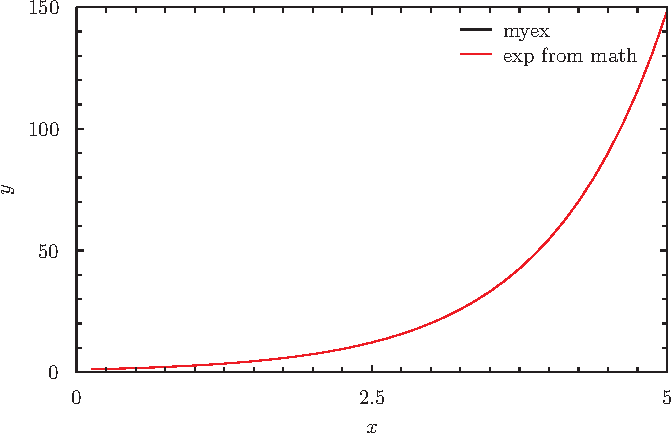
\includegraphics{fig-pyxplot.pdf}
\caption{The implemented ex-function and the exp(x) function from math}
	\end{figure}

\begin{thebibliography}{9}
\bibitem{taylor} Rudin, Walter (1987). Real and complex analysis 
(3rd ed.). New York: McGraw-Hill. p. 1. ISBN 978-0-07-054234-1.
\end{thebibliography}

\end{document}

